% ============= setup ============= %
% ======== package ======== %
\documentclass[mathserif]{beamer}
\usepackage{xeCJK}
\usepackage{graphicx}
\usepackage{xcolor}
\usepackage{setspace}
\usepackage{newtxmath}
\usepackage{listings} % 程式碼
\definecolor{codegreen}{rgb}{0,0.6,0}
\definecolor{codegray}{rgb}{0.5,0.5,0.5}
\definecolor{codepurple}{rgb}{0.58,0,0.82}
\definecolor{backcolour}{rgb}{0.95,0.95,0.92}
\lstdefinestyle{mystyle}{
    backgroundcolor=\color{backcolour},   
    commentstyle=\color{codegreen},
    keywordstyle=\color{magenta},
    numberstyle=\tiny\color{codegray},
    stringstyle=\color{codepurple},
    basicstyle=\ttfamily\footnotesize,
    breakatwhitespace=false,         
    breaklines=true,                 
    captionpos=b,                    
    keepspaces=true,                 
    numbers=left,                    
    numbersep=5pt,                  
    showspaces=false,                
    showstringspaces=false,
    showtabs=false,                  
    tabsize=2
}
\lstset{style=mystyle}

% ======== font ======== %
\setCJKmainfont{Taipei Sans TC Beta}
\setCJKsansfont{Taipei Sans TC Beta}
\AtBeginDocument{%
    \DeclareSymbolFont{pureletters}{OML}{cmm}{m}{it}%
    \SetSymbolFont{pureletters}{bold}{OML}{cmm}{b}{it}%
}
\hypersetup{
    colorlinks=true,
    linkcolor=black,
    urlcolor=blue
}

% ======== theme ======== %
\renewcommand{\baselinestretch}{1.25}
\usetheme{Madrid}
\usecolortheme{crane}
\setbeamertemplate{items}[circle]
\setbeamertemplate{section in toc}{\inserttocsectionnumber.~\inserttocsection}
\AtBeginSection[]{
    \begin{frame}
        \vfill
        \centering
        \begin{beamercolorbox}[sep=8pt,center,shadow=true,rounded=true]{title}
            \usebeamerfont{title}\insertsectionhead\par%
        \end{beamercolorbox}
        \vfill
    \end{frame}
}

% ======== data ======== %
\title{資料結構}
\author{temmie}
\date{}

% ============= setup ============= %

\begin{document}

\begin{frame}
    \titlepage
\end{frame}

\begin{frame}
    \tableofcontents
\end{frame}

\section{前言、名詞解釋}

\begin{frame}{七橋問題}
    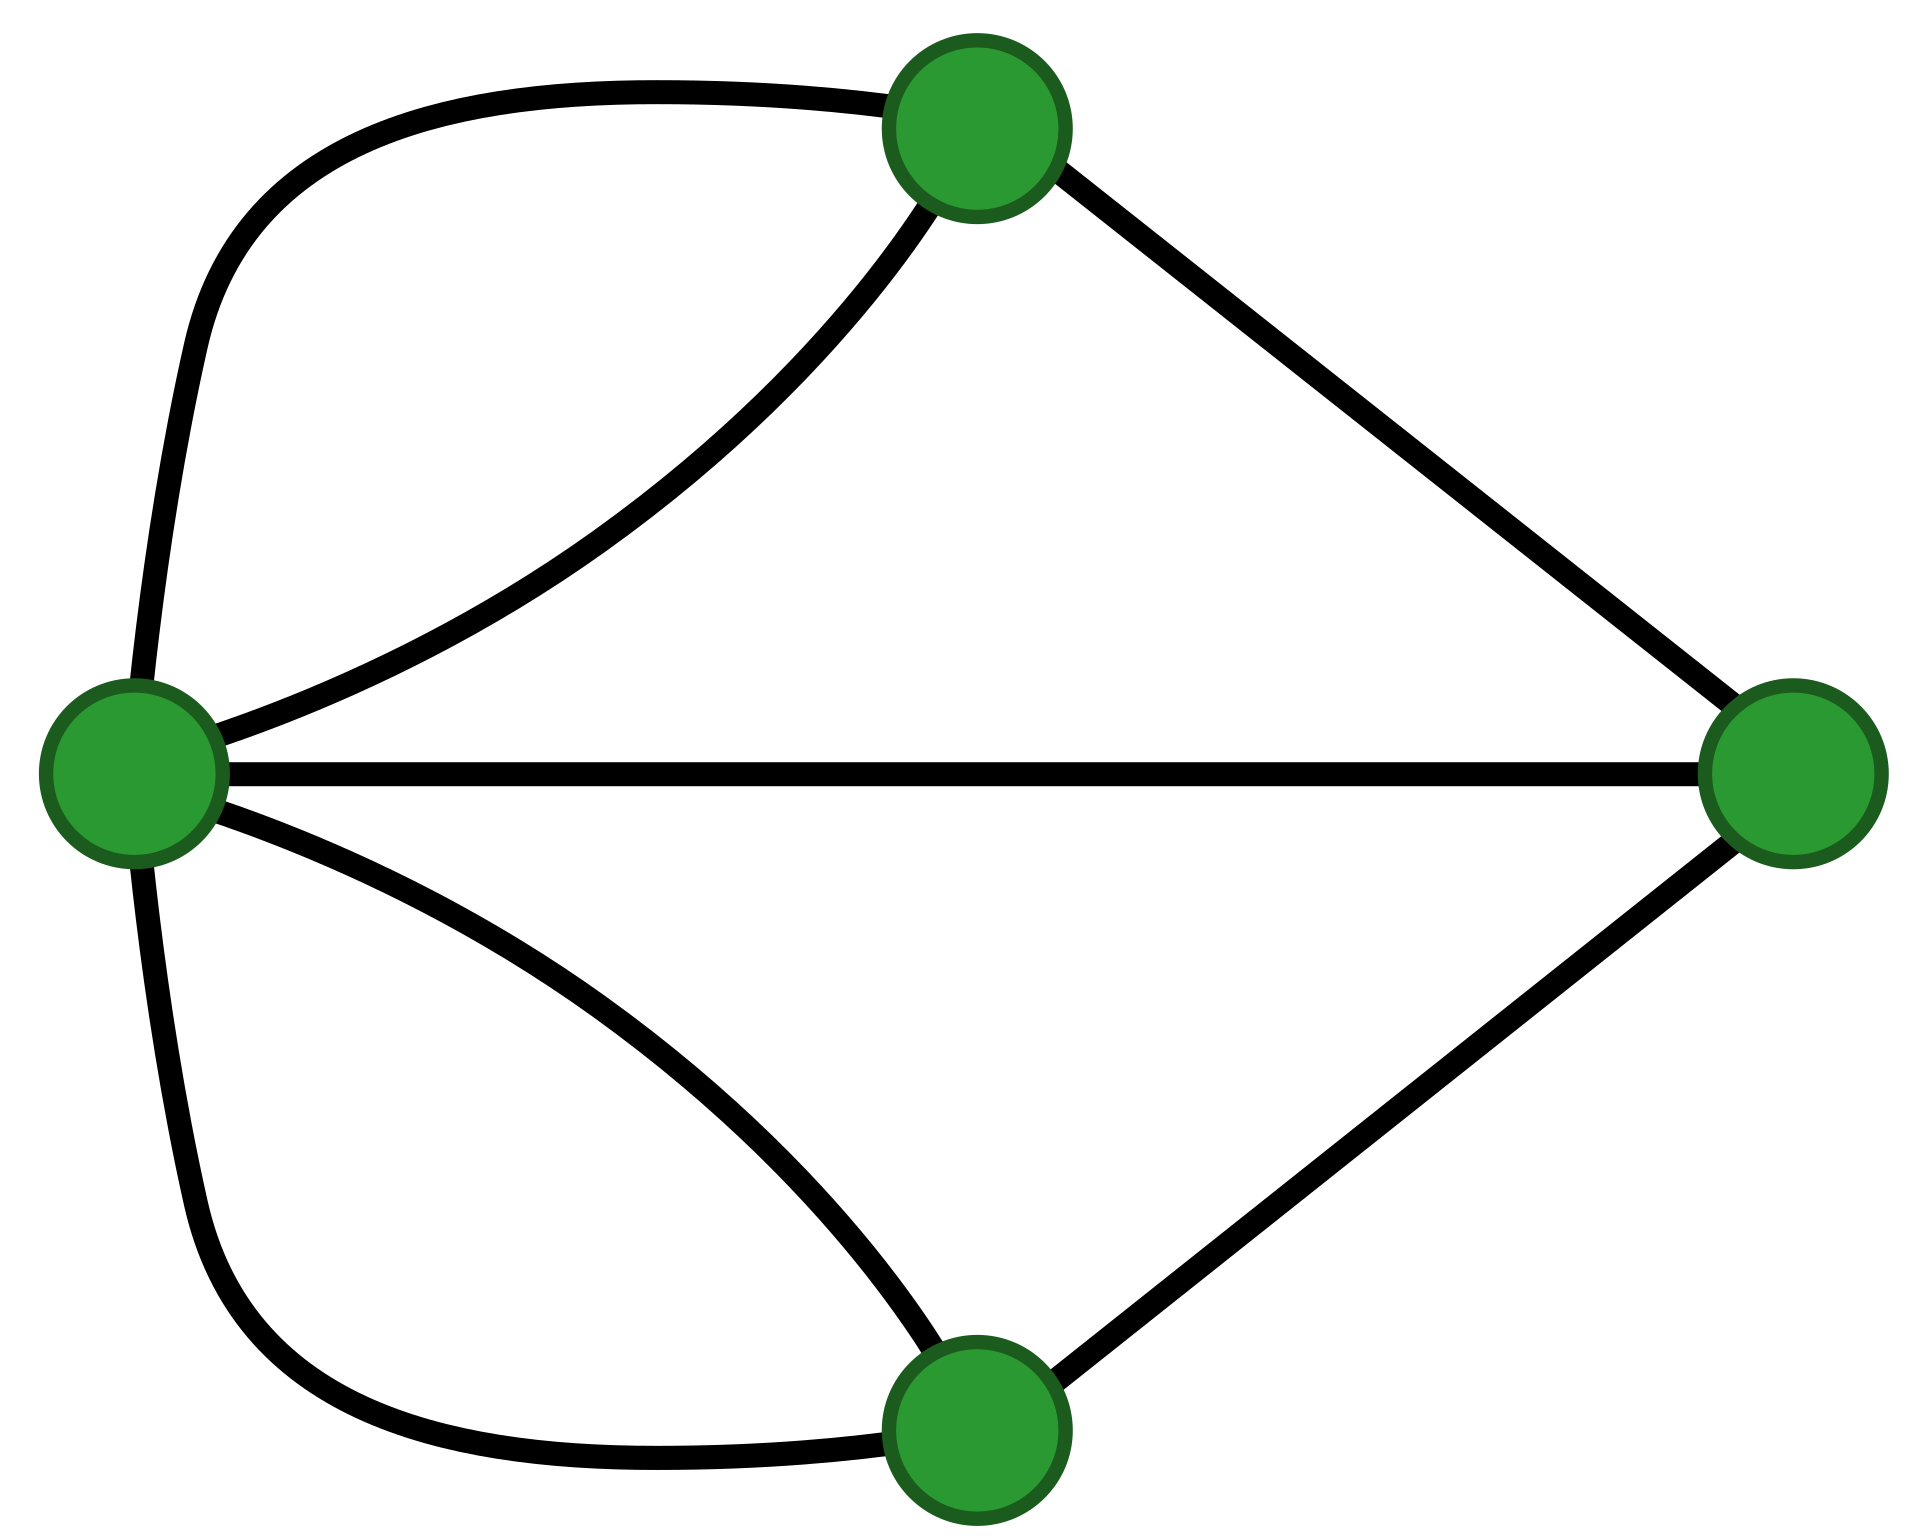
\includegraphics[width=5.0cm]{img/bridge.png}
    \begin{itemize}
        \item 有辦法經過所有的橋嗎?
        \item 上面的「圖」是怎麼構成的呢?
    \end{itemize}
\end{frame}

\begin{frame}{名詞解釋}
    \begin{itemize}
        \item 節點(Vertex,$V$)
        \item 邊(Edge,$E$):邊會將兩個節點相連
        \item 圖(Graph,$G$):由很多邊和節點組成
        \item 有向圖(Directed Graph):邊只能讓 $u$ 節點走向 $v$ 節點
        \item 無向圖(Undirected Graph):邊可以讓 $u$ 節點和 $v$ 節點互通
    \end{itemize}
\end{frame}

\begin{frame}{名詞解釋}
    \begin{itemize}
        \item 入度(In-degree,$deg^-(u)$):在有向圖中指向該節點的數量
        \item 出度(Out-degree,$deg^+(u)$):在有向圖中節點向外走的數量
        \item 度數(Degree,$deg(u)$):入度 + 出度
        \item 路徑(Path):從 $u$ 節點走向 $v$ 節點所經歷的邊
        \item 環(Cycle):從 $u$ 節點走向 $u$ 節點所經歷的邊
    \end{itemize}
\end{frame}

\section{圖的儲存}

\begin{frame}{相鄰矩陣}
    \begin{center}
        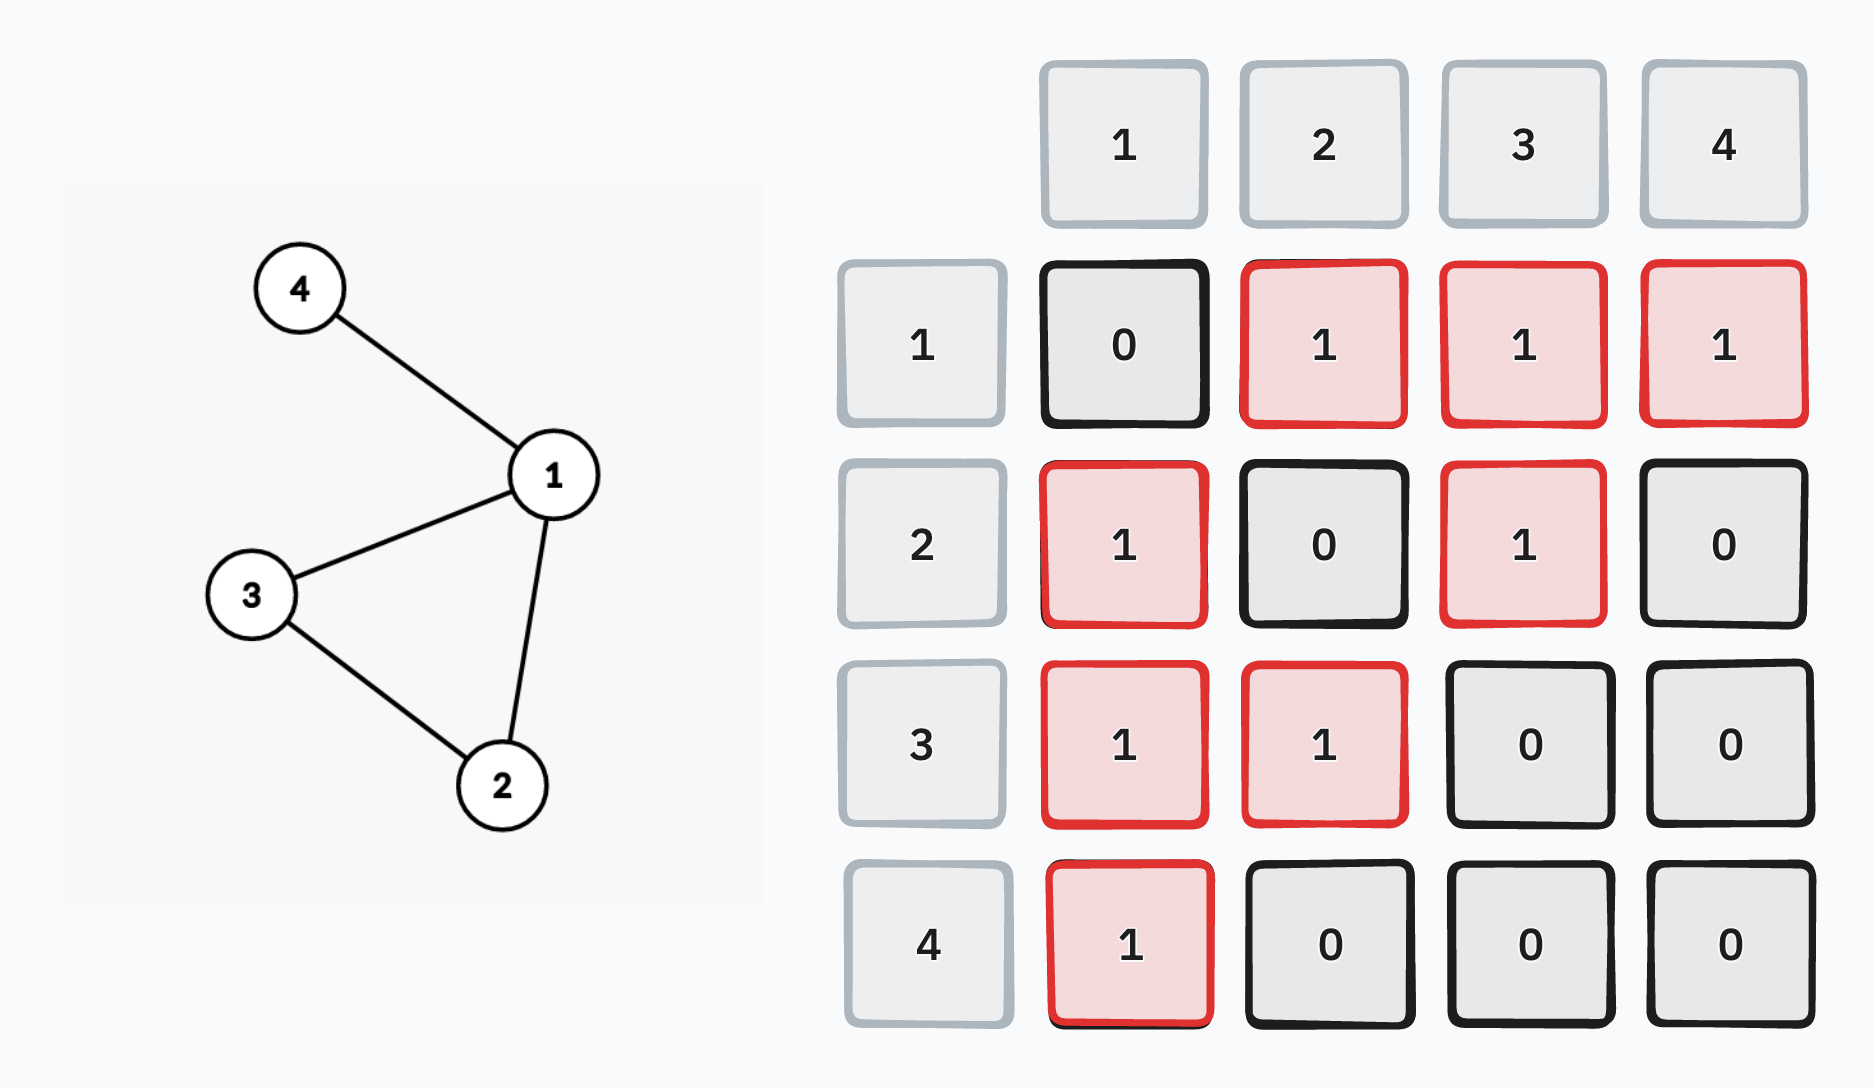
\includegraphics[width=9.0cm]{img/graph-1.png}
    \end{center}
    \begin{itemize}
        \item 尋找 $u$ 節點的所有相鄰節點:$O(V)$
        \item 遍歷整張圖:$O(V^2)$
        \item 空間複雜度:$O(V^2)$
    \end{itemize}
\end{frame}

\begin{frame}{相鄰矩陣}
    \begin{center}
        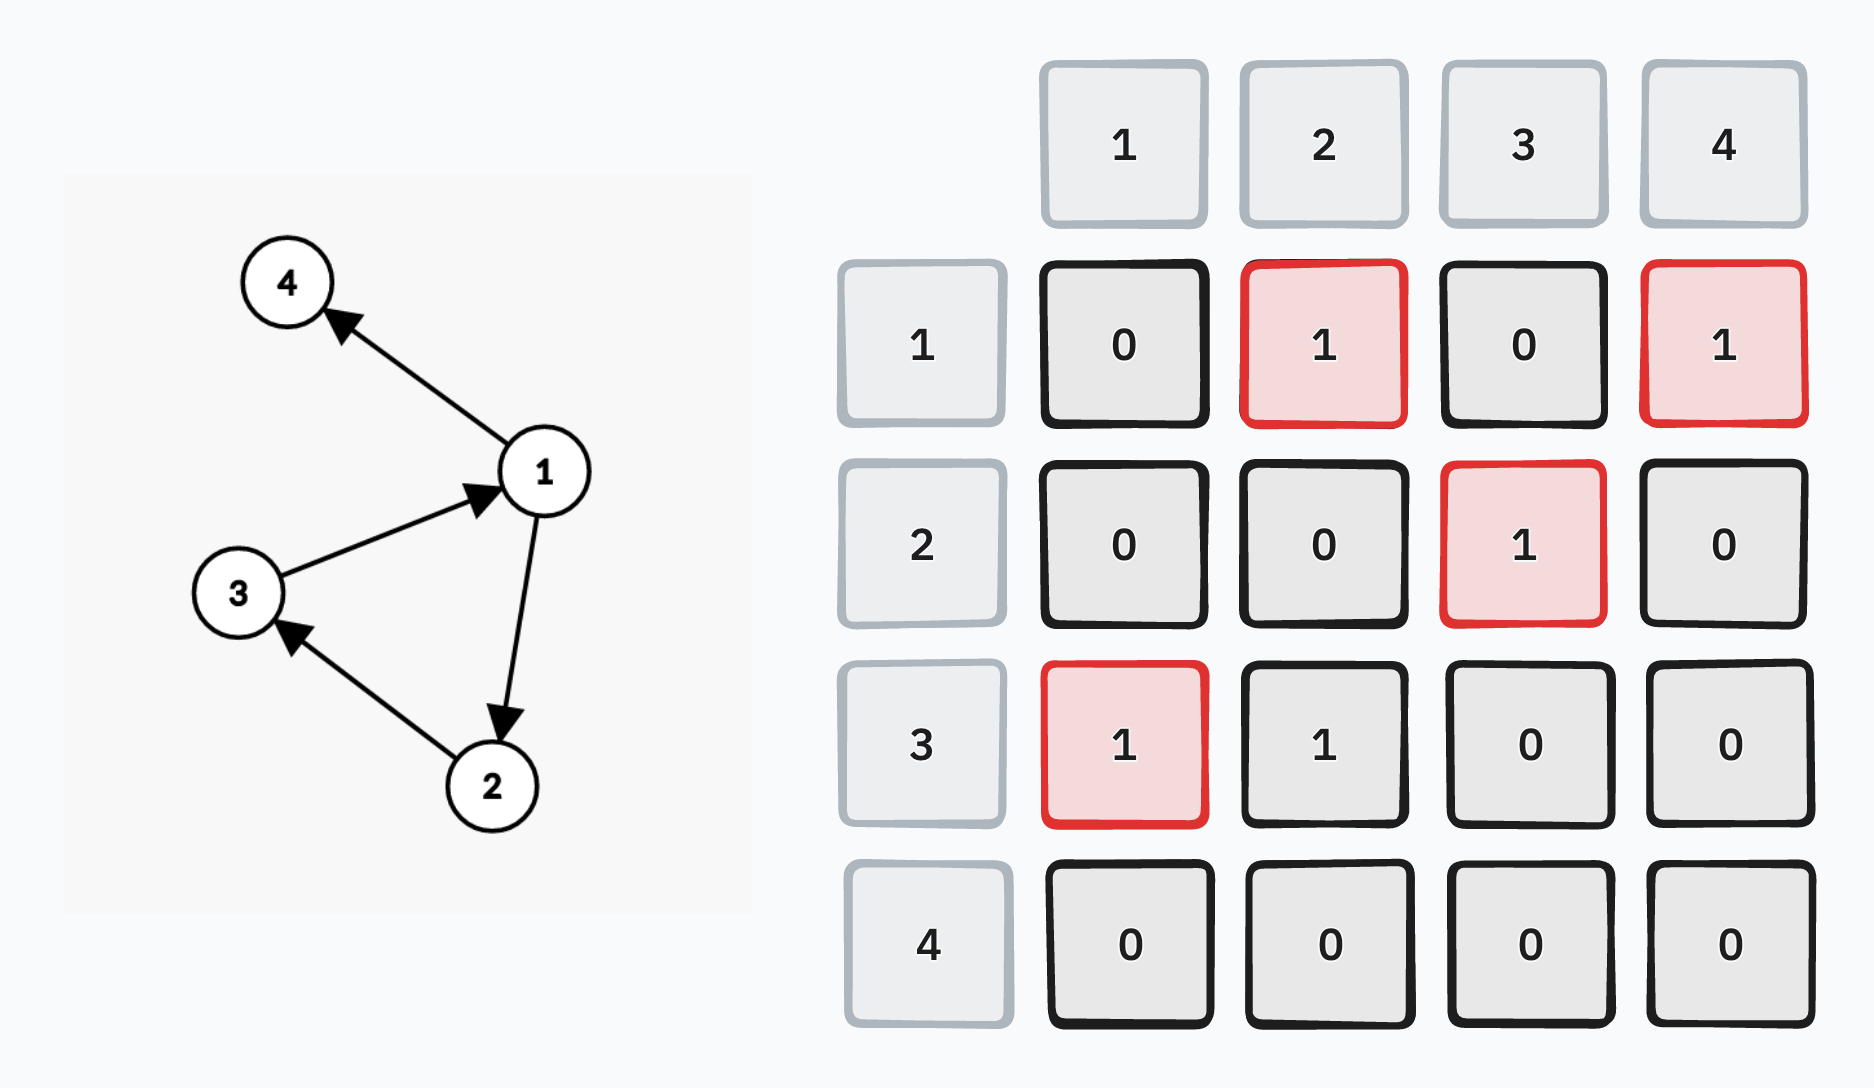
\includegraphics[width=9.0cm]{img/graph-2.png}
    \end{center}
\end{frame}

\begin{frame}{相臨串列}
    \begin{center}
        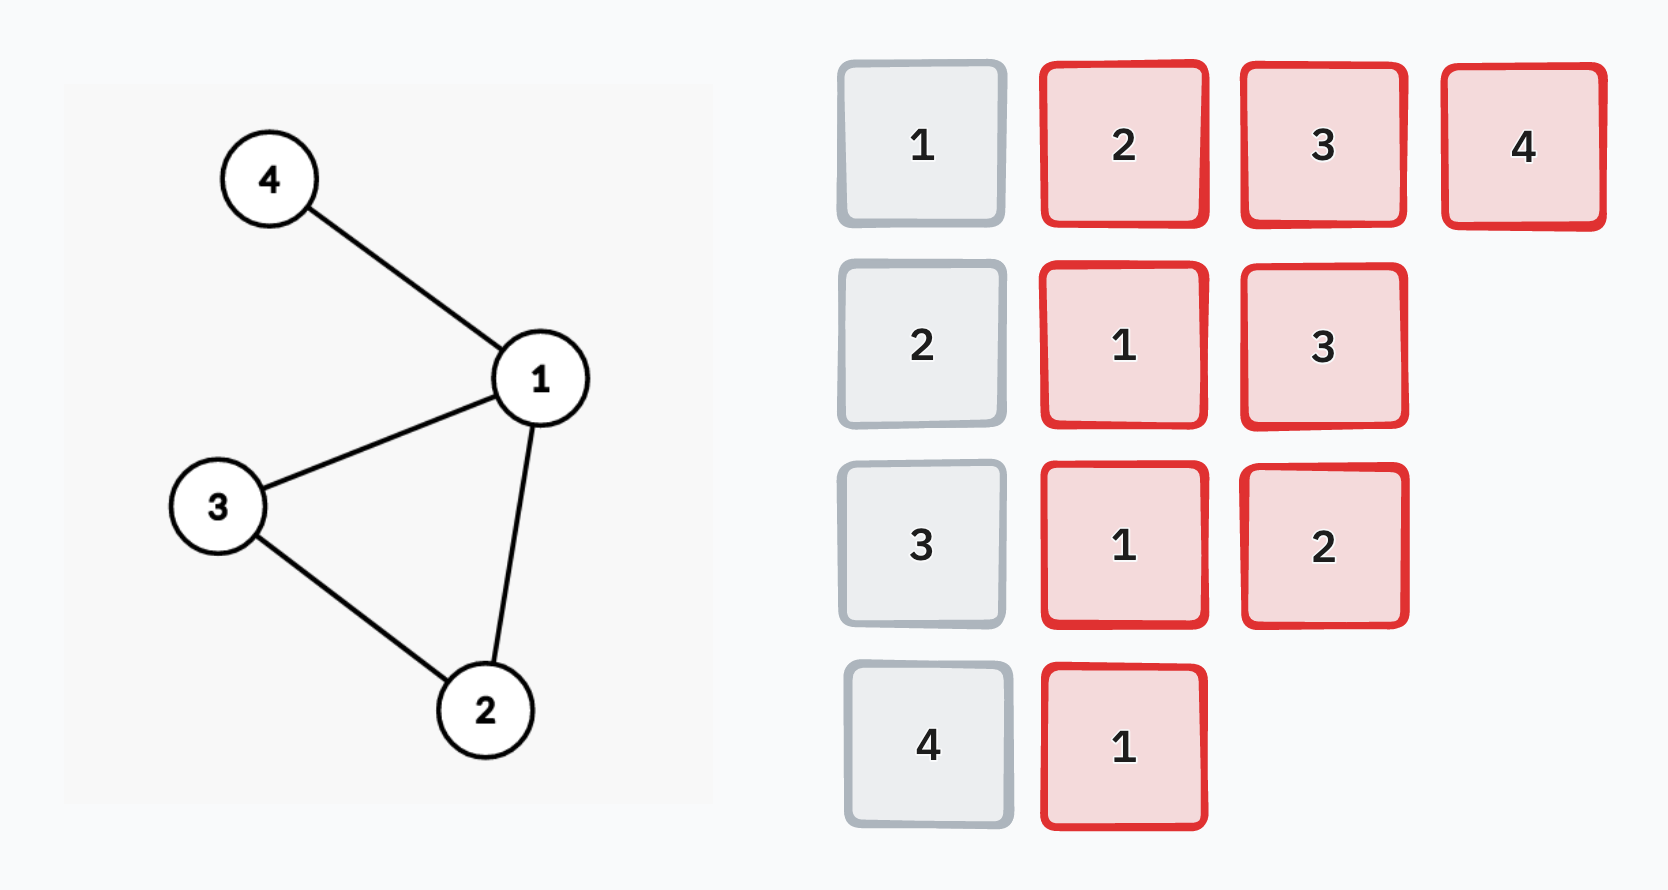
\includegraphics[width=9.0cm]{img/graph-3.png}
    \end{center}
    \begin{itemize}
        \item 尋找 $u$ 節點的所有相鄰節點:$O(deg^+)$
        \item 遍歷整張圖:$O(E)$
        \item 空間複雜度:$O(E)$
    \end{itemize}
\end{frame}

\begin{frame}{相臨串列}
    \begin{center}
        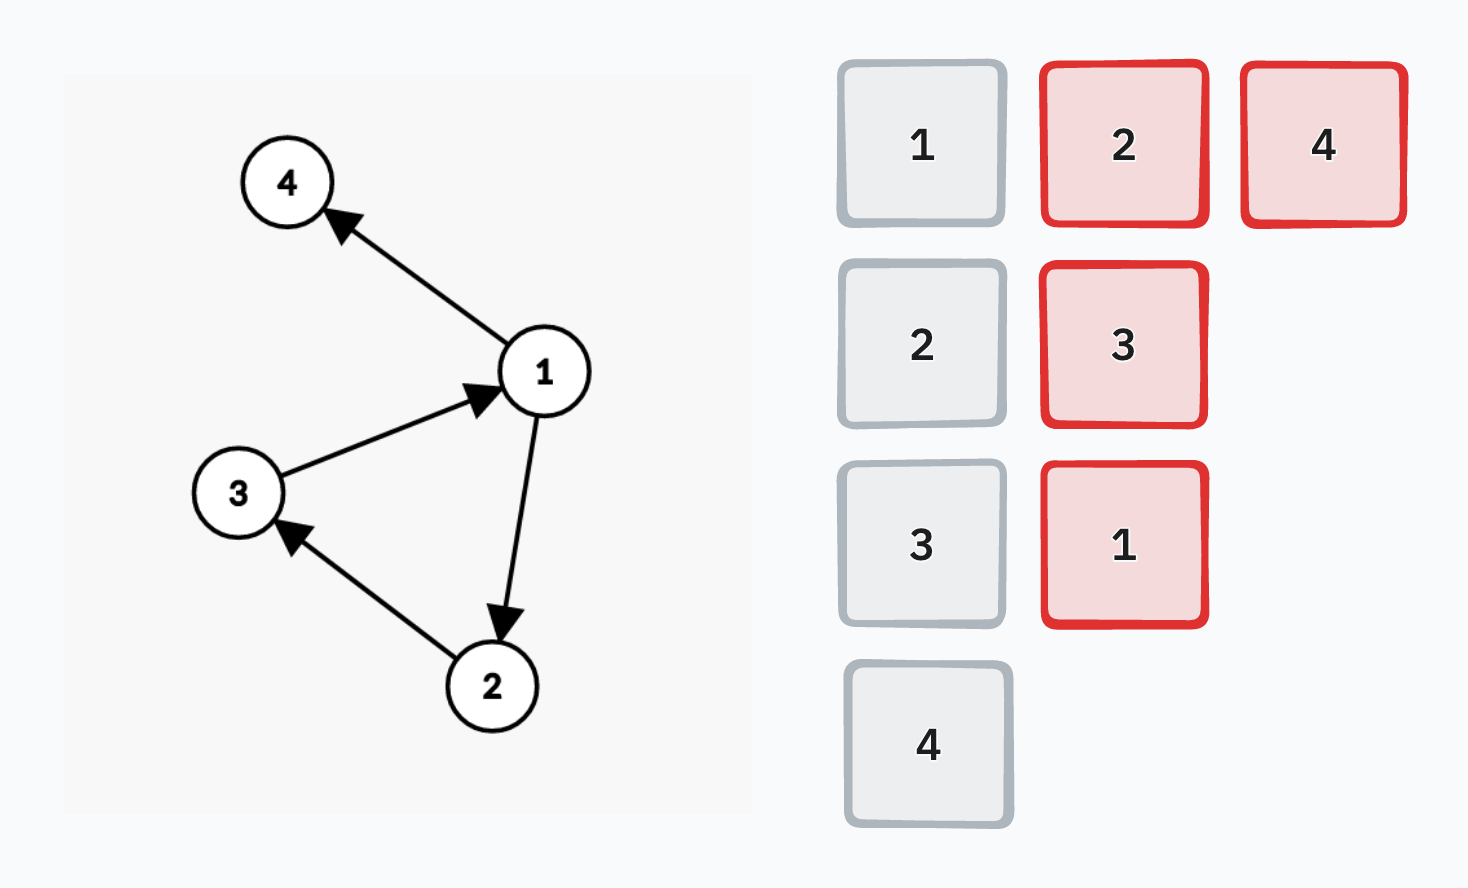
\includegraphics[width=9.0cm]{img/graph-4.png}
    \end{center}
\end{frame}

\begin{frame}[fragile]{實作:相鄰矩陣}
\begin{lstlisting}[language=C++, caption={}]
int n, m; // 有 n 個節點,m 條邊
int u, v;
int G[500][500]; // 相鄰矩陣

for (int i=0 ; i<m ; i++){
    cin >> u >> v;
    G[u][v]=1;
    // G[v][u]=1; // 如果是無向圖的話就加上此行
}
    \end{lstlisting}
\end{frame}

\begin{frame}[fragile]{實作:相鄰串列}
    \begin{lstlisting}[language=C++, caption={}]
int n, m; // 有 n 個節點,m 條邊
int u, v;
vector<vector<int>> G(500); // 相鄰串列

for (int i=0 ; i<m ; i++){
    cin >> u >> v;
    G[u].push_back(v);
    // G[v].push_back(u); // 如果是無向圖的話就加上此行
}
\end{lstlisting}
\end{frame}

\section{DFS}

\begin{frame}{DFS}
    \begin{itemize}
        \item 深度優先搜尋(Depth-First-Search,DFS),一種遍歷圖的方法
        \item 顧名思義:我們會將\textbf{深度作為最先搜尋的對象}
        \item 步驟如下
            \begin{enumerate}
                \itemsep=5pt
                \item 選擇起點當作\textbf{目前的節點}
                \item 紀錄目前的節點走過
                \item 前往其中一個沒走過的相鄰節點當作目前的節點
                \item 如果全部的相鄰節點都走完就將目前的節點設為父節點
                \item 如果所有節點都走過就結束
            \end{enumerate}
    \end{itemize}
\end{frame}

\begin{frame}{DFS}
    \begin{itemize}
        \item 讓我們以這張圖做個例子
        \item 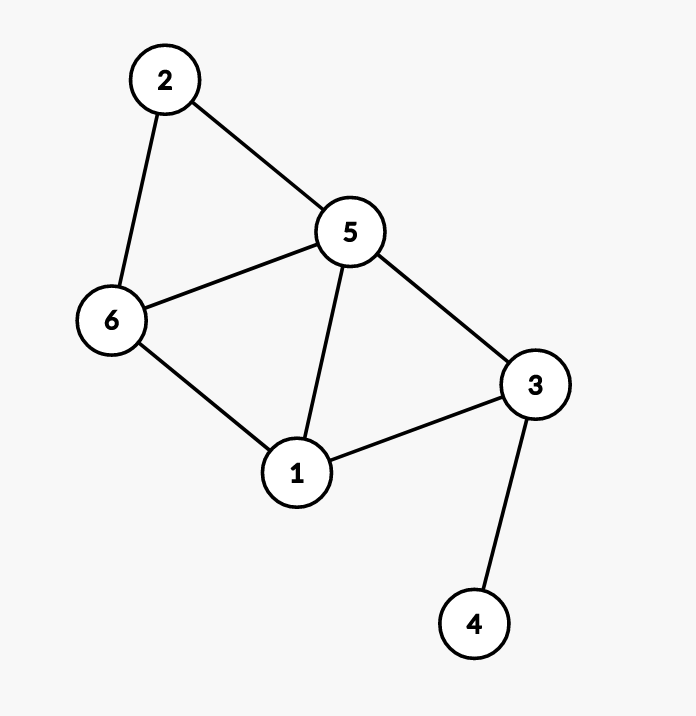
\includegraphics[width=6.0cm]{img/graph-5.png}
    \end{itemize}
\end{frame}

\begin{frame}[fragile]{實作:DFS}
\begin{lstlisting}[language=C++, caption={}]
vector<vector<int>> G(500); // 相鄰串列
bitset<500> vis; // 紀錄是否走過第 i 點

void dfs(int now){
    vis[now]=1; // 2. 紀錄目前的節點走過
    for (auto x : G[now]){
        if (vis[x]==0){ // 3. 前往沒走過的相鄰節點
            dfs(x);
        }
    }
    return; // 4. 全部的相鄰節點都走完就將目前節點設為父節點
}

dfs(1); // 1. 選擇起點當作目前節點
\end{lstlisting}
\end{frame}

\begin{frame}{例題}
    \begin{block}{Building Roads}
        \href{https://cses.fi/problemset/task/1666}{題目連結}

        有 $n$ 個城市 $m$ 條道路,請問需要新增幾條道路才能讓所有城市連通。

        請輸出數量以及新增的道路。

    \end{block}
    \begin{itemize}
        \item<2-> Tip1:已經有連通的城市還需要新增道路嗎?
        \item<3-> Tip2:兩個不連通的程式要新增幾條道路才能連通?
    \end{itemize}
\end{frame}


\begin{frame}[fragile]{例題}
\begin{lstlisting}[language=C++, caption={}]
vector<int> ans;

for (int i=1 ; i<=n ; i++){
    // 一個城市還沒被遍歷,就記錄他並且走過所有跟他連通的城市
    if (vis[i]){
        ans.push_back(i);
        dfs(i);
    }
}

cout << ans.size()-1 << "\n";
for (int i=0 ; i<ans.size()-1 ; i++){
    cout << ans[i] << " " << ans[i+1] << "\n";
}
\end{lstlisting}
\end{frame}


\begin{frame}{例題}
    \begin{block}{Counting Rooms}
        \href{https://cses.fi/problemset/task/1192}{題目連結}

        給你一個大小為 $n \times m$ 的房間,\textbf{@} 代表為地板,\textbf{#} 代表為牆壁,在一個地板上可以上下左右走向另一個地板,並視為在同一個房間。
        
        請問房間的數量?
    \end{block}
    \begin{itemize}
        \item<2-> Tip1:請先想想看,這要怎麼轉換成一張圖呢?
        \item<3-> Tip2:這是一個二維的平面,請問該如何表示目前的節點?
    \end{itemize}
\end{frame}

\begin{frame}[fragile]{例題}
\begin{lstlisting}[language=C++, caption={}]
bool vis[1005][1005];

bool out(int x, int y){ // 檢查下一個座標是否出界
    return x<0 || x>n || y<0 || y>m;
}

void dfs(int x, int y){
    vis[x][y]=1;
    if (out(x+1, y)==0 && v[x+1][y]=='.') dfs(x+1, y);
    if (out(x-1, y)==0 && v[x-1][y]=='.') dfs(x-1, y);
    if (out(x, y+1)==0 && v[x][y+1]=='.') dfs(x, y+1);
    if (out(x, y-1)==0 && v[x][y-1]=='.') dfs(x, y-1);
    return;
}
\end{lstlisting}
\end{frame}

\begin{frame}[fragile]{例題}
\begin{lstlisting}[language=C++, caption={}]
bool vis[1005][1005];
const int mx[4]={1, 0, -1, 0};
const int my[4]={0, 1, 0, -1};

bool out(int x, int y){ // 檢查下一個座標是否出界
    return x<0 || x>n || y<0 || y>m;
}

void dfs(int x, int y){
    vis[x][y]=1;
    for (int i=0 ; i<4 ; i++){
        if (out(x+mx[i], y+my[i])==0 &&
        v[x+mx[i]][y+my[i]]=='.') dfs(x+mx[i], y+my[i]);
    }
    return;
}
\end{lstlisting}
\end{frame}

\section{BFS}

\begin{frame}{BFS}
    \begin{itemize}
        \item 深度優先搜尋(Breadth-First-Search,BFS),一種遍歷圖的方法
        \item 同樣地,會以廣度為最優先的順序。
        \item 步驟如下
            \begin{enumerate}
                \itemsep=5pt
                \item 選擇起點當作目前的節點,\textbf{紀錄走過}後將處理順序設為 1
                \item 紀錄目前的節點走過
                \item 將所有相鄰節點依序紀錄處理順序後,\textbf{並直接紀錄走過}
                \item 尋找下一個處理順序的節點
                \item 如果所有節點都走過就結束,否則重複第二步驟
            \end{enumerate}
    \end{itemize}
\end{frame}

\begin{frame}{比較}
    \begin{itemize}
        \item DFS 跟 BFS 都可以遍歷整張圖
        \item DFS 相對更好實作,也比較方便一些動態規劃的題目
        \item BFS 比較難實作一些,不過擁有了\textbf{最短路}的性質
    \end{itemize}
\end{frame}

\section{回朔解}

\begin{frame}{回朔解}
    \begin{itemize}
        \item 在一些問題中,題目將會要求構造出一種解法。
        \item 這個問題我們可以透過\textbf{逆推}達成。
        \item 也就是紀錄\textbf{這個結果是由誰推過來的}
    \end{itemize}
\end{frame}

\begin{frame}{例題}
    \begin{block}{CLabyrinth}
        \href{https://cses.fi/problemset/task/1193}{題目連結}

        給你一個大小為 $n \times m$ 的房間,\textbf{@} 代表為地板,\textbf{#} 代表為牆壁,在一個地板上可以上下左右走向另一個地板,並且給予一個點 \textbf{A} 代表起點,\textbf{B} 代表終點。\\
        \vspace{1em}
        請判斷是否有辦法從起點走向終點,如果可以,則輸出 \textbf{"Yes"},並且輸出\textbf{最短路徑長度}以及用 \textbf{LRUD} 代表\textbf{左右上下}構造一任意一組解。
    \end{block}
    \begin{itemize}
        \item<2-> Tip1:怎麼知道是否有辦法從起點走到終點?
        \item<3-> Tip2:如果是最短路徑,那們要用 DFS 還是 BFS ?
        \item<4-> Tip3:如果知道 $A$ 是從 $B$ 轉移的話,要怎麼紀錄資訊進行反推?
    \end{itemize}
\end{frame}

\begin{frame}[fragile]{例題}
\begin{lstlisting}[language=C++, caption={}]
int parent[1005][1005];

void dfs(int x, int y){
    vis[x][y]=1;
    for (int i=0 ; i<4 ; i++){
        if (out(x+mx[i], y+my[i])==0 &&
        v[x+mx[i]][y+my[i]]=='.'){
            
            dfs(x+mx[i], y+my[i]);
        }
    }
    return;
}
\end{lstlisting}
\end{frame}


\end{document}